

\tikzset{every picture/.style={line width=0.75pt}} %set default line width to 0.75pt        

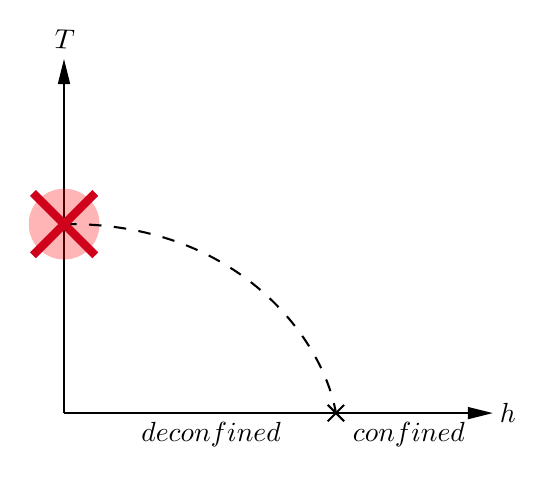
\begin{tikzpicture}[x=0.75pt,y=0.75pt,yscale=-1,xscale=1]
%uncomment if require: \path (0,300); %set diagram left start at 0, and has height of 300

%Straight Lines [id:da6058174087985544] 
\draw    (155.33,248.33) -- (359.89,248.33) ;
\draw [shift={(361.89,248.33)}, rotate = 180] [fill={rgb, 255:red, 0; green, 0; blue, 0 }  ][line width=0.08]  [draw opacity=0] (12,-3) -- (0,0) -- (12,3) -- cycle    ;
%Straight Lines [id:da3876935202277678] 
\draw    (155.33,248.33) -- (155.33,79.85) ;
\draw [shift={(155.33,77.85)}, rotate = 450] [fill={rgb, 255:red, 0; green, 0; blue, 0 }  ][line width=0.08]  [draw opacity=0] (12,-3) -- (0,0) -- (12,3) -- cycle    ;
%Straight Lines [id:da6788890136308154] 
\draw    (286.33,248.33) ;
\draw [shift={(286.33,248.33)}, rotate = 45] [color={rgb, 255:red, 0; green, 0; blue, 0 }  ][line width=0.75]    (-5.59,0) -- (5.59,0)(0,5.59) -- (0,-5.59)   ;
%Shape: Circle [id:dp6881434470754835] 
\draw  [draw opacity=0][fill={rgb, 255:red, 255; green, 0; blue, 0 }  ,fill opacity=0.29 ] (138.33,157.28) .. controls (138.33,147.86) and (145.97,140.22) .. (155.39,140.22) .. controls (164.81,140.22) and (172.44,147.86) .. (172.44,157.28) .. controls (172.44,166.7) and (164.81,174.33) .. (155.39,174.33) .. controls (145.97,174.33) and (138.33,166.7) .. (138.33,157.28) -- cycle ;
%Curve Lines [id:da9144656520027832] 
\draw  [dash pattern={on 4.5pt off 4.5pt}]  (155.39,157.28) .. controls (239.89,156.22) and (280.56,213.56) .. (286.33,248.33) ;
%Straight Lines [id:da7908951123243328] 
\draw [color={rgb, 255:red, 208; green, 2; blue, 27 }  ,draw opacity=1 ][line width=3]    (155.39,157.28) ;
\draw [shift={(155.39,157.28)}, rotate = 45] [color={rgb, 255:red, 208; green, 2; blue, 27 }  ,draw opacity=1 ][line width=3]    (-21.24,0) -- (21.24,0)(0,21.24) -- (0,-21.24)   ;

% Text Node
\draw (363.89,248.33) node [anchor=west] [inner sep=0.75pt]    {$h$};
% Text Node
\draw (155.45,74.45) node [anchor=south] [inner sep=0.75pt]  [rotate=-2]  {$T$};
% Text Node
\draw (226.17,251.4) node [anchor=north] [inner sep=0.75pt]    {$\text{deconfined}$};
% Text Node
\draw (321.5,251.4) node [anchor=north] [inner sep=0.75pt]    {$\text{confined}$};


\end{tikzpicture}
